\documentclass[aps,onecolumn,nofootinbib,pra]{article}

\usepackage{../../spec_files/arxiv}
\input{../../spec_files/standard_preamble.tex}

\input{../../macros/organization_macros.tex}
\newcommand{\var}[1]{\text{\emph{#1}}}

\newcommand{\synencodingof}[1]{S\left(#1\right)} % Syntax encoding!
\newcommand{\stringof}[1]{\textit{"#1"}}

\newcommand{\rdf}{\mathrm{RDF}}
\newcommand{\mathrdftype}{\mathrm{rdf}\mathrm{type}}
\newcommand{\rdftype}{$\mathrm{rdf}:\mathrm{type}$}

\newcommand{\zerotuple}[1]{0_{#1}}
\newcommand{\onetuple}[1]{1_{#1}}

\newcommand{\truesymbol}{\mathrm{True}}
\newcommand{\falsesymbol}{\mathrm{False}}
\newcommand{\truthset}{\{\falsesymbol,\truesymbol\}}
\newcommand{\truthstate}{z}
\newcommand{\truthstateof}[1]{\truthstate_{#1}}
\newcommand{\ozset}{\{0,1\}}
\newcommand{\ozbasisset}{\{\fbasisat{\catvariable},\tbasisat{\catvariable}\}}

\newcommand{\setwithout}[2]{#1\backslash#2}
\newcommand{\setexcept}[1]{\backslash#1}
\newcommand{\whileSymbol}{$\mathrm{while}$}

\newcommand{\modspace}{\,\,\,\mathrm{mod}\,\,}

\newcommand{\uniquantwrtof}[2]{\forall{#1}:{#2}}
\newcommand{\existquantwrtof}[2]{\exists{#1}:{#2}}
\newcommand{\imppremhead}[2]{\left(#1\right)\Rightarrow\left(#2\right)}

\newenvironment{centeredscript}% Use for tnreason script language, lstlistings for python code!
{\begin{center}
     \begin{algorithmic}
         \hspace{1cm}}
{\end{algorithmic}\end{center}}

\newcommand{\inlinecode}[1]{\lstinline[language=Python]|#1|}

\newcommand{\algdefsymbol}{\leftarrow}
\newcommand{\proofrightsymbol}{"$\Rightarrow$"}
\newcommand{\proofleftsymbol}{"$\Leftarrow$"}
\newcommand{\defcols}{\,:\,} % in definitions of functions
\newcommand{\wcols}{\,:\,} % in definitions of sets
\newcommand{\ncond}{,\,} %next cond
\newcommand{\defspace}{\quad,\quad}
\newcommand{\andspace}{\quad\text{and}\quad}
\newcommand{\ifspace}{\text{if}\quad}
\newcommand{\elsetext}{\text{else}}
\newcommand{\stspace}{\quad \text{subject to} \quad}

\newcommand{\iosepline}{\vspace{0.5em} \hrule \vspace{0.5em}}

\newcommand{\distassymbol}{\sim}
\newcommand{\probtagtypeinst}[2]{\mathrm{P}^{#1}_{#2}}

\newcommand{\mprojectionsymbol}{\mathrm{M}}
\newcommand{\iprojectionsymbol}{\mathrm{I}}
\newcommand{\gainsymbol}{\mathrm{gain}}
\newcommand{\gradientsymbol}{\mathrm{grad}}
\newcommand{\greedysymbol}{\mathrm{greedy}}
\newcommand{\hubosymbol}{\mathrm{HUBO}}
\newcommand{\maximizationsymbol}{\mathrm{max}}

% Entropies
\newcommand{\entropysymbol}{\mathbb{H}}
\newcommand{\sentropyof}[1]{\entropysymbol\left[#1\right]}
\newcommand{\sentropyofwrt}[2]{\entropysymbol_{#2}\left[#1\right]}
\newcommand{\centropyof}[2]{\entropysymbol\left[#1,#2\right]}
\newcommand{\centropyofwrt}[3]{\entropysymbol_{#3}\left[#1,#2\right]}
\newcommand{\kldivsymbol}{\mathrm{D}_{\mathrm{KL}}}
\newcommand{\kldivof}[2]{\kldivsymbol\left[ #1 || #2 \right]}
\newcommand{\mutinfof}[2]{I\left(#1;#2\right)}
\newcommand{\condmutinfof}[3]{\mutinfof{#1}{#2|#3}}
\newcommand{\subspacedimof}[1]{\mathrm{dim}(#1)}

\newcommand{\subsphere}{\mathbb{S}}
\newcommand{\rr}{\mathbb{R}}
\newcommand{\nn}{\mathbb{N}}

\newcommand{\closureof}[1]{\overline{#1}}
\newcommand{\interiorof}[1]{{#1}^{\circ}}
\newcommand{\sbinteriorof}[1]{{\left(#1\right)}^{\circ}}

\newcommand{\difofwrt}[2]{\frac{\partial #1}{\partial #2}}
\newcommand{\difwrt}[1]{\difofwrt{}{#1}}
\newcommand{\gradwrt}[1]{\nabla_{#1}}
\newcommand{\gradwrtat}[2]{\nabla_{#1}|_{#2}}

\newcommand{\cardof}[1]{\left|#1\right|}
\newcommand{\absof}[1]{\left|#1\right|}

\newcommand{\imageof}[1]{\mathrm{im}\left(#1\right)}

\newcommand{\convhullof}[1]{\mathrm{conv}\left(#1\right)}
\newcommand{\cubeof}[1]{[0,1]^{#1}}
\newcommand{\dimof}[1]{\mathrm{dim}\left(#1\right)}
\newcommand{\spanof}[1]{\mathrm{span}\left(#1\right)}
\newcommand{\subspaceof}[1]{V^{#1}}

\newcommand{\argmin}{\mathrm{argmin}}
\newcommand{\argmax}{\mathrm{argmax}}

% Help functions
\newcommand{\chainingfunction}{h}
\newcommand{\chainingfunctionof}[1]{\chainingfunction\left(#1\right)}

\newcommand{\greaterthanfunction}[1]{\ones_{>#1}}
\newcommand{\greaterthanfunctionof}[2]{\greaterthanfunction{#1}\left(#2\right)}
\newcommand{\existquanttrafo}{\greaterthanfunction{0}}
\newcommand{\universalquanttrafo}{\greaterthanfunction{\inddim-1}}

\newcommand{\greaterzerofunction}{\greaterthanfunction{0}}
\newcommand{\greaterzeroof}[1]{\greaterzerofunction\left(#1\right)}
\newcommand{\equalzeroof}[1]{\ones_{\{0\}}\left(#1\right)}
\newcommand{\equaloneof}[1]{\ones_{\{0\}}\left(#1\right)}

\newcommand{\nonzerofunction}{\ones_{\neq0}}
\newcommand{\nonzeroof}[1]{\nonzerofunction\left(#1\right)}
\newcommand{\nonzerocirc}{\nonzerofunction\circ}

\newcommand{\valof}[1]{\mathrm{val}\left(#1\right)}

% Probability distributions
\newcommand{\expof}[1]{\mathrm{exp}\left[#1\right]}
\newcommand{\probtensor}{\mathbb{P}}
\newcommand{\probtensorof}[1]{\probtensor^{#1}}
\newcommand{\probtensorofat}[2]{\probtensor^{#1}\left[#2\right]}
\newcommand{\secprobtensor}{\tilde{\mathbb{P}}}
\newcommand{\secprobat}[1]{\secprobtensor[#1]}
\newcommand{\secprobwith}{\secprobat{\shortcatvariables}}

\newcommand{\probfamilyofat}[3]{\probofat{#1}{#2|#3}}
\newcommand{\membervariable}{Z}
\newcommand{\memberindex}{z}
\newcommand{\indexedmembervariable}{\membervariable=\memberindex}
\newcommand{\probfamilywith}{\probfamilyof{}{\shortcatvariables}{\membervariable}}

\newcommand{\independent}[2]{\left(#1\perp#2\right)}
\newcommand{\condindependent}[3]{\left(#1\perp#2\middle)\,\right|\,#3}

\newcommand{\probtensorset}{\Gamma}
\newcommand{\probtensorin}{\probtensor\in\probtensorset}
\newcommand{\bmrealprobof}[1]{\realizabledistsof{\identity,\maxgraph,#1}}%
\newcommand{\alldists}{\realizabledistsof{\identity,\maxgraph}}

\newcommand{\gendistribution}{\probtensor^*}
\newcommand{\gendistributionat}[1]{\gendistribution\left[#1\right]}
\newcommand{\gendistributionwith}{\gendistributionat{\shortcatvariables}}
\newcommand{\currentdistribution}{\tilde{\probtensor}}
\newcommand{\currentdistributionat}[1]{\currentdistribution\left[#1\right]}
\newcommand{\currentdistributionwith}{\currentdistributionat{\shortcatvariables}}

\newcommand{\probat}[1]{\probtensor\left[#1\right]}
\newcommand{\probof}[1]{\probtensor^{#1}}
\newcommand{\probofat}[2]{\probof{#1}\left[#2\right]}
\newcommand{\probwith}{\probat{\shortcatvariables}}
\newcommand{\probwithnodes}{\probat{\nodevariables}}
\newcommand{\probofwrt}[2]{\probtensor_{#1}\left[#2\right]}

\newcommand{\condprobat}[2]{\mathbb{P}\big[#1\big|#2\big]}
\newcommand{\condprobof}[2]{\condprobat{#1}{#2}}
\newcommand{\condprobwrtof}[3]{\mathbb{P}^{#1}\big[#2\big|#3\big]}
\newcommand{\margprobat}[1]{\probat{#1}}
\newcommand{\expectationof}[1]{\mathbb{E}\left[#1\right]}
\newcommand{\expectationofwrt}[2]{\mathbb{E}_{#2}\left[#1\right]}
\newcommand{\lnof}[1]{\ln \left[ #1 \right] }
\newcommand{\sgnormof}[1]{\left\|#1\right\|_{\psi_2}} % subgaussian
\newcommand{\normof}[1]{\left\|#1\right\|_{2}}

\newcommand{\sinof}[1]{\mathrm{sin}\left(#1\right)}
\newcommand{\cosof}[1]{\mathrm{cos}\left(#1\right)}

\newcommand{\ones}{\mathbb{I}}
\newcommand{\onesof}[1]{\ones^{#1}}
\newcommand{\onesat}[1]{\ones\left[#1\right]}
\newcommand{\onesofat}[2]{\onesof{#1}\left[#2\right]}
\newcommand{\oneswith}{\onesat{\shortcatvariables}}
\newcommand{\zeros}{0}
\newcommand{\zerosat}[1]{\zeros\left[#1\right]}
\newcommand{\identity}{\dirdelta}
\newcommand{\identityat}[1]{\identity\left[#1\right]}

\newcommand{\bernoulliof}[1]{B(#1)}

\newcommand{\deltaof}[1]{\delta_{#1}} % used in coordinate calculus proofs

\newcommand{\indicatorof}[1]{\ones_{#1}}
\newcommand{\indicatorofat}[2]{\ones_{#1}\left[#2\right]}

\newcommand{\exmatrix}{M}
\newcommand{\matrixat}[1]{\exmatrix[#1]}
\newcommand{\matrixofat}[2]{\exmatrix^{#1}\left[#2\right]}

\newcommand{\exvector}{V}
\newcommand{\vectorof}[1]{\exvector^{#1}}
\newcommand{\vectorat}[1]{\exvector[#1]}
\newcommand{\vectorofat}[2]{\exvector^{#1}[#2]}

\newcommand{\restrictionofto}[2]{{#1}|_{#2}}
\newcommand{\restrictionoftoat}[3]{\restrictionofto{#1}{#2}\left[#3\right]}

\newcommand{\idsymbol}{\mathrm{Id}} % ! Different to delta tensor in \identity
\newcommand{\idrestrictedto}[1]{\restrictionofto{\idsymbol}{#1}}

%% KNOWLEDGE GRAPH
\newcommand{\kg}{\mathrm{KG}|_{\worldindices}}
\newcommand{\kgat}[1]{\kg\left[#1\right]}
\newcommand{\kgreptensor}{\bencodingof{\kg}}

\newcommand{\exaunaryrelation}{C}
\newcommand{\exabinaryrelation}{R}

\newcommand{\kgtriple}[3]{\braket{#1,#2,#3}}
\newcommand{\exunarytriple}{\kgtriple{\provariable}{\mathrdftype}{\exaunaryrelation}}
\newcommand{\exbinarytriple}{\kgtriple{\provariableof{0}}{\exabinaryrelation}{\provariableof{1}}}

\newcommand{\atomcreator}{\psi}
\newcommand{\atomcreatorofat}[2]{\atomcreator_{#1}\left[#2\right]}
\newcommand{\provariable}{Z}
\newcommand{\provariableof}[1]{\provariable_{#1}}

\newcommand{\sparql}{\mathrm{SPARQL}}
\newcommand{\joinsymbol}{\mathrm{JOIN}}

\newcommand{\subsymbol}{s}
\newcommand{\predsymbol}{p}
\newcommand{\objsymbol}{o}

\newcommand{\sindvariable}{\indvariableof{\subsymbol}}
\newcommand{\pindvariable}{\indvariableof{\predsymbol}}
\newcommand{\oindvariable}{\indvariableof{\objsymbol}}

\newcommand{\invrdftypesymbol}{\mathrm{typ}}



 % Hard leg set to a given dimension




\newcommand{\extractionrelation}{\exrelation}

\newcommand{\variableset}{A} % Still used in monomial decomposition, NOT for object sets! -> Use \hardlegset instead!
\newcommand{\variablesetof}[1]{\variableset^{#1}}

\newcommand{\formulaset}{\mathcal{F}}
\newcommand{\formulasetof}[1]{\formulaset_{#1}}

\newcommand{\secformulaset}{\tilde{\formulaset}}

\newcommand{\hardformulaset}{\kb}
\newcommand{\hfbasemeasure}{\basemeasureof{\hardformulaset}}
\newcommand{\hfbasemeasureat}[1]{\hfbasemeasure\left[#1\right]}
\newcommand{\softformulaset}{\formulaset}


% Formula Selecting
\newcommand{\larchitecture}{\mathcal{A}}
\newcommand{\larchitectureat}[1]{\larchitecture\left[#1\right]}

\newcommand{\inneuronset}{\mathcal{A}^{\mathrm{in}}}
\newcommand{\outneuronset}{\mathcal{A}^{\mathrm{out}}}

\newcommand{\lneuron}{\mathcal{N}}
\newcommand{\lneuronof}[1]{\lneuron_{#1}}
\newcommand{\lneuronat}[1]{\lneuron\left(#1\right)}
\newcommand{\lneuractivation}{\sencodingof{\lneuron}}
\newcommand{\lneuractivationat}[1]{\lneuractivation\left[#1\right]}

\newcommand{\fsnn}{\sencodingof{\larchitecture}}
\newcommand{\fsnnat}[1]{\fsnn\left[#1\right]}

\newcommand{\sliceselectionmapof}[1]{\sencodingof{\fselectionmapof{\land,#1}}}
\newcommand{\sliceselectionmapofat}[2]{\sliceselectionmapof{#1}\left[#2\right]}
\newcommand{\sliceselectionmapat}[1]{\sliceselectionmapofat{\catorder,\sliceorder}{#1}}

\newcommand{\skeleton}{S}
\newcommand{\skeletonof}[1]{\skeleton\left(#1\right)}
\newcommand{\skeletontensor}{\bencodingof{\skeleton}} %OLD! Use skeleton

\newcommand{\skeletoncore}{S}
\newcommand{\skeletoncoreof}[1]{\skeletoncore^{#1}}

\newcommand{\cselectionsymbol}{C}
\newcommand{\vselectionsymbol}{V}
\newcommand{\sselectionsymbol}{S}

\newcommand{\selinputvariable}{\selvariable}
\newcommand{\cselinputvariable}{\selvariableof{\cselectionsymbol}}
\newcommand{\vselinputvariable}{\selvariableof{\vselectionsymbol}}

\newcommand{\fselectionmap}{\hlnstat}
\newcommand{\fselectionmapof}[1]{\fselectionmap_{#1}}
\newcommand{\fselectionmapat}[1]{\fselectionmap\left(#1\right)}
\newcommand{\fselectionmapofat}[2]{\fselectionmap_{#1}\left(#2\right)}

\newcommand{\sencfselectionmap}{\sencodingof{\fselectionmap}}
\newcommand{\sencfselectionmapat}[1]{\sencfselectionmap\left[#1\right]}

\newcommand{\cselectionmap}{\fselectionmapof{\cselectionsymbol}}
\newcommand{\cselectionmapat}[1]{\fselectionmapofat{\cselectionsymbol}{#1}}

\newcommand{\senccselectionmap}{\sencodingof{\cselectionmap}}
\newcommand{\senccselectionmapat}[1]{\senccselectionmap\left[#1\right]}

\newcommand{\vselectionmap}{\fselectionmapof{\vselectionsymbol}}
\newcommand{\vselectionmapat}[1]{\fselectionmapofat{\vselectionsymbol}{#1}}
\newcommand{\vselectionheadvar}{\headvariableof{\vselectionsymbol}} % Replacing \catvariableof{\vselectionmap}

\newcommand{\sencvselectionmap}{\sencodingof{\vselectionmap}}
\newcommand{\sencvselectionmapat}[1]{\sencvselectionmap\left[#1\right]}

\newcommand{\sselectionmap}{\fselectionmapof{\sselectionsymbol}}
\newcommand{\sselectionmapat}[1]{\fselectionmapofat{\sselectionsymbol}{#1}}

\newcommand{\sencsselectionmapat}[1]{\sencodingofat{\fselectionmapof{\sselectionsymbol}}{#1}}

\newcommand{\vselectionmapof}[1]{\fselectionmapof{\vselectionsymbol,#1}} % tb deleted!

\newcommand{\tranfselectionmap}{\fselectionmap^T}

% Output variables - Following the catvariable convention
\newcommand{\seloutputvariable}{\catvariable}
\newcommand{\cseloutputvariable}{\catvariableof{\cselectionsymbol}}
\newcommand{\vseloutputvariable}{\headvariableof{\vselectionsymbol}}

% Tensor Core Representation
\newcommand{\selectorcore}{{\bsencodingof{\vselectionsymbol}}}
\newcommand{\selectorcoreof}[1]{\bsencodingof{\vselectionmapof{#1}}}

\newcommand{\selectorcomponentof}[1]{\hypercoreof{{#1}}} % Since not an basis encoding!
\newcommand{\selectorcomponentofat}[2]{\selectorcomponentof{#1}\left[#2\right]}

\newcommand{\parspace}{\rr^{\seldim}}
\newcommand{\fullparcube}{[0,1]^{\seldim}}
\newcommand{\boundaryparcube}{\{0,1\}^{\seldim}} % ! This is not the boundary of the cube
\newcommand{\parcubevertices}{\{0,1\}^{\seldim}}
\newcommand{\cubeface}{Q}

\newcommand{\cubefaceparam}{\variableset,\headindexof{\variableset}}

\newcommand{\unitvectoratof}[2]{e^{(#1)}_{#2}}
\newcommand{\parametrizingunittensor}{e_{\atomindices}} % Not required?



%% OPTIMIZATION
\newcommand{\targettensor}{\energytensor}
\newcommand{\importancetensor}{I}

%% MARKOV LOGIC NETWORK
\newcommand{\loss}{\mathcal{L}_{\datamap}}
\newcommand{\lossof}[1]{\loss\left(#1\right)}
\newcommand{\mlnformulaset}{\mathcal{F}}
\newcommand{\mlnformulain}{\exformula\in\mlnformulaset}
\newcommand{\weight}{\theta}
\newcommand{\weightof}[1]{\weight_{#1}}
\newcommand{\weightat}[1]{\weight[#1]}

\newcommand{\mlnparameters}{\formulaset,\canparam}
\newcommand{\mlntrueparameters}{(\formulaset^*,\weight^*)}



% Examples
\newcommand{\mlnatomsymbol}{[\catorder]}
\newcommand{\mlnmintermsymbol}{\land}
\newcommand{\mlnmaxtermsymbol}{\lor}

\newcommand{\partitionfunction}{\mathcal{Z}}
\newcommand{\secpartitionfunction}{\tilde{\mathcal{Z}}}
\newcommand{\partitionfunctionof}[1]{\partitionfunction\left(#1\right)}
\newcommand{\secpartitionfunctionof}[1]{\secpartitionfunction\left(#1\right)}

\newcommand{\mlnprob}{\probtensorof{\mlnparameters}}
\newcommand{\mlnprobat}[1]{\expdistofat{\mlnparameters}{#1}}
\newcommand{\mlnenergy}{\energytensorof{\mlnparameters}}

\newcommand{\folmlnparameters}{\folformulastat,\canparam,\basemeasureof{\fixedimpformula}}
\newcommand{\folhlnparameters}{\folformulastat,\hybridparam}
% For Probabilistic Analysis



\newcommand{\mintermnoise}{\noiseof{\identity}}
\newcommand{\mlnnoise}{\noiseof{\hlnstat}}
\newcommand{\mlnnoiseat}[1]{\mlnnoise\left[#1\right]}

\newcommand{\fprob}{p} % Drop! This is mean parameter
\newcommand{\fprobof}[1]{\fprob^{(#1)}}

\newcommand{\bidistof}[1]{B\left(#1\right)}
\newcommand{\multidistof}[1]{\underline{B}\left(#1\right)}
\newcommand{\widthwrtof}[2]{\Omega_{#1}\left(#2\right)}
\newcommand{\widthatof}[2]{\widthwrtof{#1}{#2}}

\newcommand{\selbasisshort}{\Gamma}
\newcommand{\selbasislong}{\{\onehotmapofat{\selindex}{\selvariable} \,:\, \selindexin \}}

\newcommand{\failprob}{u}
\newcommand{\precision}{t}
\newcommand{\maxgap}{\Delta}
\newcommand{\maxgapofat}[2]{\maxgap_{#1}\left(#2\right)}
\newcommand{\maxgapof}[1]{\maxgap\left(#1\right)}

\newcommand{\invtemp}{\beta}

\newcommand{\extnetasset}{\left\{\hypercoreofat{\edge}{\catvariableof{\edge}}\wcols\edgein\right\}}

\newcommand{\singlecanparam}{\canparam}

\newcommand{\seccanparam}{\tilde{\canparam}}
\newcommand{\seccanparamat}[1]{\seccanparam\left[#1\right]}

\newcommand{\canparamwrtat}[2]{\canparamofat{#1}{#2}}
\newcommand{\estcanparam}{\hat{\canparam}}
\newcommand{\naivecanparam}{\tilde{\canparam}}
\newcommand{\naivecanparamat}[1]{\naivecanparam\left[#1\right]}

\newcommand{\datacanparam}{\canparamof{\datamap}}
\newcommand{\datacanparamat}[1]{\canparamofat{\datamap}{#1}}

\newcommand{\gencanparam}{\canparamof{*}}
\newcommand{\gencanparamat}[1]{\canparamofat{*}{#1}}

\newcommand{\canmetric}{d}
\newcommand{\canmetricwrt}[1]{\canmetric_{#1}}
\newcommand{\canmetricwrtof}[3]{\canmetric_{#1}\left(#2,#3\right)}
\newcommand{\canmetricof}[2]{\canmetric\left(#1,#2\right)}


\newcommand{\canparamhypothesis}{\Gamma}
\newcommand{\canparamin}{\canparam\in\canparamhypothesis}

\newcommand{\greedyhypothesis}{\mathcal{H}}

\newcommand{\energyhypothesis}{\Theta}
\newcommand{\energyhypothesisof}[1]{\energyhypothesis^{#1}}




%% Factored System


\newcommand{\statevectorof}[1]{v_{#1}}
\newcommand{\statevectorofat}[2]{\statevectorof{#1}\left[#2\right]}

% Greedy
\newcommand{\extendedformulaset}{\formulaset\cup\{\formula\}}
\newcommand{\extendedcanparam}{\tilde{\canparam}\cup\{\weightof{\formula}\}}

\newcommand{\exfunction}{q}
\newcommand{\exfunctionof}[1]{\exfunction_{#1}}
\newcommand{\exfunctiontargetspace}{\bigotimes_{l\in[p]}\rr^{\catdimof{l}}}
\newcommand{\exfunctiontargetvariables}{Y_0,\ldots,Y_{p-1}}
\newcommand{\exfunctionimageelement}{y}
\newcommand{\exfunctionat}[1]{\exfunction(#1)}
\newcommand{\exfunctionofat}[2]{\exfunctionof{#1}(#2)}
\newcommand{\secexfunction}{g}
\newcommand{\secexfunctionat}[1]{\secexfunction(#1)}
\newcommand{\secexfunctionof}[1]{\secexfunction^{#1}}

\newcommand{\realvaluedfunction}{\exfunction}
\newcommand{\realvaluedfunctionev}[1]{\realvaluedfunction\left(#1\right)} % Evaluated
\newcommand{\realvaluedfunctionat}[1]{\realvaluedfunction\left[#1\right]}

\newcommand{\statesetfunction}{\exfunction}
\newcommand{\statesetfunctionev}[1]{\statesetfunction\left(#1\right)}

\newcommand{\tenvaluedfunction}{\exfunction}
\newcommand{\tenvaluedfunctionev}[1]{\tenvaluedfunction\left(#1\right)}
\newcommand{\tenvaluedfunctionat}[1]{\tenvaluedfunction\left[#1\right]}

\newcommand{\compositionof}[2]{{#1}\circ{#2}}
\newcommand{\compositionofat}[3]{(\compositionof{#1}{#2})(#3)}

%% Message Passing
\newcommand{\scheduler}{S}
\newcommand{\ovgraph}{\graph^{\mathrm{overlap}}} % overlap graph to the hypergraph
\newcommand{\dirovgraph}{\graph^{\rightarrow}} % directed overlap graph
\newcommand{\ovedges}{\edges^{\mathrm{overlap}}}
\newcommand{\dirovedges}{\edges^{\rightarrow}}

\newcommand{\sedge}{\edgeof{0}} % Send edge
\newcommand{\redge}{\edgeof{1}} % Receive edge
\newcommand{\secsedge}{\edgeof{2}}
\newcommand{\thirdsedge}{\edgeof{3}}

\newcommand{\preedgesetwrt}[2]{\edges^{\rightarrow(#1,#2)}}
\newcommand{\preedgeset}{\preedgesetwrt{\sedge}{\redge}}

\newcommand{\cluster}{C}
\newcommand{\clusterof}[1]{\cluster_{#1}}
\newcommand{\clusterenumerator}{i}
\newcommand{\secclusterenumerator}{j}
\newcommand{\thirdclusterenumerator}{\tilde{j}}

\newcommand{\enc}{\clusterof{\clusterenumerator}}
\newcommand{\secenc}{\clusterof{\secclusterenumerator}}
\newcommand{\thirdenc}{\clusterof{\thirdclusterenumerator}}

\newcommand{\clusterorder}{n}
\newcommand{\clusterenumeratorin}{\clusterenumerator\in[\clusterorder]}

\newcommand{\updatedmesfromtowith}[2]{\hat{\messagesymbol}_{#1 \rightarrow #2}\left[\catvariableof{#1 \cap #2}\right]}

\newcommand{\upmes}[2]{\delta_{#1 \rightarrow #2}}
\newcommand{\downmes}[2]{\delta_{#2 \leftarrow #1}}

% Binary connective symbols
\newcommand{\impbincon}{\Rightarrow}
\newcommand{\eqbincon}{\Leftrightarrow}
\newcommand{\lpasbincon}{\triangleleft}

\newcommand{\notucon}{\lnot}
\newcommand{\iducon}{\mathrm{Id}}
\newcommand{\trueucon}{\mathrm{T}}

\newcommand{\woneoplus}{\bigoplus^{(1)}}
\newcommand{\modsumsymbol}{\tilde{+}}
\newcommand{\marysumsymbol}{+^{\catdim}}

\newcommand{\indexinterpretation}{I}
\newcommand{\indexinterpretationof}[1]{\indexinterpretation_{#1}}
\newcommand{\indexinterpretationat}[1]{\indexinterpretation\left[#1\right]}
\newcommand{\indexinterpretationofat}[2]{\indexinterpretationof{#1}\left[#2\right]}

\newcommand{\indinttensorofat}[2]{\indexinterpretationof{#1}\left[#2\right]}

\newcommand{\invindexinterpretation}{\indexinterpretation^{-1}}
\newcommand{\invindexinterpretationof}[1]{\indexinterpretation_{#1}^{-1}}
\newcommand{\invindexinterpretationat}[1]{\invindexinterpretation(#1)}
\newcommand{\invindexinterpretationofat}[2]{\invindexinterpretationof{#1}(#2)}

%ILP
\newcommand{\objectivesymbol}{c}
\newcommand{\objofat}[2]{\objectivesymbol^{#1}\left[#2\right]}
\newcommand{\rhssymbol}{b}
\newcommand{\rhsofat}[2]{\rhssymbol^{#1}\left[#2\right]}

% Coordinate Calculus
\newcommand{\coordinatetrafowrtof}[2]{{#1}\left(#2\right)}
\newcommand{\coordinatetrafowrtofat}[3]{\coordinatetrafowrtof{#1}{#2}\left[#3\right]}

\newcommand{\linmap}{F}
\newcommand{\linmapof}[1]{\linmap^{#1}}
\newcommand{\linmapofat}[2]{\linmapof{#1}\left(#2\right)}
\newcommand{\linmapspace}{\mathbb{L}}

%% Directed Tensor Calculus
\newcommand{\exrelation}{\mathcal{R}}
\newcommand{\exrelationof}[1]{\exrelation^{#1}}
\newcommand{\arbset}{\mathcal{U}}
\newcommand{\arbsetof}[1]{\arbset^{#1}}
\newcommand{\arbsubset}{\mathcal{V}} % Conflicts with nodes!
\newcommand{\arbelement}{u}
\newcommand{\arbelementin}{\arbelement\in\arbset}

\newcommand{\insymbol}{\mathrm{in}}
\newcommand{\outsymbol}{\mathrm{out}}
\newcommand{\midsymbol}{\mathrm{mid}}
\newcommand{\inset}{\arbsetof{\insymbol}}
\newcommand{\outset}{\arbsetof{\outsymbol}}

\newcommand{\incatindex}{\catindexof{\insymbol}}
\newcommand{\outcatindex}{\catindexof{\outsymbol}}

%% Sparse Tensor Calculus
\newcommand{\sparsityof}[1]{\ell_0\left(#1\right)}

\newcommand{\sudokunum}{n}
\newcommand{\sudokustartevidence}{E^{\mathrm{start}}}
\newcommand{\sudokukbof}[1]{\kb^{#1}}


%% Book

\newcommand{\messageedge}{\edgeof{m}}
\newcommand{\inferenceedges}{\edgesof{\mathrm{inference}}}
\newcommand{\coloredmatrixof}[2]{\begin{pmatrix}
#1
\end{pmatrix}\left[#2\right]}
\newcommand{\blankmatrix}[1]{\begin{pmatrix}
#1
\end{pmatrix}}



%% ENCODING SCHEMES: Coordinate, basis, selection
\newcommand{\cencodingof}[1]{\chi^{#1}}
\newcommand{\cencodingofat}[2]{\cencodingof{#1}\left[#2\right]}
\newcommand{\cencodingwith}{\cencodingofat{\exfunction}{\shortcatvariables}}

\newcommand{\bencodingof}[1]{\beta^{#1}}
\newcommand{\bencodingofat}[2]{\bencodingof{#1}\left[#2\right]}
\newcommand{\bencodingwith}{\bencodingofat{\exfunction}{\headvariableof{\exfunction},\shortcatvariables}}

\newcommand{\sencodingof}[1]{\sigma^{#1}}
\newcommand{\sencodingofat}[2]{\sencodingof{#1}\left[#2\right]}
\newcommand{\sencodingwith}{\sencodingofat{\exfunction}{\shortcatvariables,\selvariable}}

\newcommand{\bsencodingof}[1]{\bencodingof{\sencodingof{#1}}} % {\bencodingof{#1}}% % Following the convention at the end of notation chapter
\newcommand{\bsencodingofat}[2]{\bencodingofat{\sencodingof{#1}}{#2}} % {\bencodingofat{#1}{#2}}%

\newcommand{\brepresentationof}[1]{\tau^{#1}}
\newcommand{\brepresentationofat}[2]{\brepresentationof{#1}\left[#2\right]}





% Missing: \omega (weights)

%% Sets of tensors
\newcommand{\expfamilyof}[1]{\Gamma^{#1}}
\newcommand{\expfamily}{\genexpfamily}
\newcommand{\genexpfamily}{\expfamilyof{\sstat,\basemeasure}}
\newcommand{\expfamilywith}{\expfamilyof{\sstat,\basemeasure}}

\newcommand{\realizabledistsof}[1]{\Lambda^{#1}}
\newcommand{\maxrealizabledistsof}[1]{\realizabledistsof{#1,\maxgraph}}
\newcommand{\elrealizabledistsof}[1]{\realizabledistsof{#1,\elformat}}
\newcommand{\realizabledistswith}{\realizabledistsof{\sstat,\graph}}
\newcommand{\hlnsetof}[1]{\realizabledistsof{#1,\elformat}}

\newcommand{\cansof}[1]{\Lambda^{#1}}
\newcommand{\maxtrivcansof}[1]{\Lambda^{#1,\maxgraph,\trivbm}}
\newcommand{\eltrivcansof}[1]{\Lambda^{#1,\elformat,\trivbm}}



%% Cores
\newcommand{\categoricalmap}{e}
\newcommand{\categoricalmapat}[1]{\categoricalmap\left(#1\right)}
\newcommand{\categoricalmapof}[1]{\categoricalmap^{#1}}
\newcommand{\categoricalmapofat}[2]{\categoricalmap^{#1}\left(#2\right)}

\newcommand{\categoricalcore}{\bencodingof{\categoricalmap}}
\newcommand{\categoricalcoreof}[1]{\bencodingof{\categoricalmapof{#1}}}
\newcommand{\categoricalcoreat}[1]{\bencodingof{\categoricalmap}\left[#1\right]}
\newcommand{\categoricalcoreofat}[2]{\bencodingof{\categoricalmapof{#1}}\left[#2\right]}

\newcommand{\datamap}{D}
\newcommand{\datamapat}[1]{\datamap(#1)}
\newcommand{\datamapof}[1]{\datamap_{#1}}
\newcommand{\datapointof}[1]{\datamapat{#1}}
\newcommand{\datapoint}{\datapointof{\datindex}}
\newcommand{\dataset}{\left((\catindicesof{\datindex})\,:\,\datindexin\right)}

\newcommand{\secdatamap}{\tilde{\datamap}}
\newcommand{\datacore}{\bencodingof{\datamap}}
\newcommand{\datacoreat}[1]{\datacore\left[#1\right]}
\newcommand{\datacoreof}[1]{\bencodingof{\datamap_{#1}}}
\newcommand{\datacoreofat}[2]{\bencodingof{\datamap_{#1}}[#2]}

\newcommand{\secdatacoreof}[1]{\bencodingof{\secdatamap_{#1}}}
\newcommand{\empdistribution}{\probtensor^{\datamap}}
\newcommand{\empdistributionat}[1]{\empdistribution\left[#1\right]}
\newcommand{\empdistributionwith}{\empdistributionat{\shortcatvariables}}

\newcommand{\varcore}[1]{U^{#1}} % For optimization of tensor network
\newcommand{\varspace}[1]{\rr^{p_{#1}}}
\newcommand{\varcollection}{\big\{\varcore{\atomenumerator}\, :\, \atomenumeratorin \big\}}

% DecompositionIndex 
\newcommand{\decvariable}{I}
\newcommand{\decvariableof}[1]{\decvariable_{#1}}
\newcommand{\decindex}{i} % Needs to be different to datindex!
\newcommand{\decindexof}[1]{\decindex_{#1}}
\newcommand{\indexeddecvariableof}[1]{\decvariableof{#1}=\decindexof{#1}}
\newcommand{\decdim}{n}
\newcommand{\decdimof}[1]{\decdim_{#1}}
\newcommand{\decindexin}{\decindex\in[\decdim]}
\newcommand{\indexeddecvariable}{\decvariable=\decindex}
\newcommand{\inddecvar}{\indexeddecvariable}

\newcommand{\indexeddatvariable}{\datvariable=\datindex}

% Used in poly sparsity
\newcommand{\indexvariable}{\datvariable} % for datacores used
\newcommand{\indexset}{J}
\newcommand{\indexsetof}[1]{\indexset^{#1}}

\newcommand{\slackvariable}{z}
\newcommand{\slackindex}{z}
\newcommand{\slackindexof}[1]{\slackindex_{#1}}

\newcommand{\rankofat}[2]{\mathrm{rank}^{#1}\left(#2\right)}
\newcommand{\cprankof}[1]{\mathrm{rank}\left(#1\right)}
\newcommand{\bincprankof}[1]{\mathrm{rank}^{\mathrm{bin}}\left(#1\right)}
\newcommand{\polsparsityof}[1]{\slicerankwrtof{\catorder}{#1}} % former {\tilde{\ell} \left(#1\right)}


\newcommand{\dircprankof}[1]{\mathrm{rank}^{\mathrm{dir}}\left(#1\right)}
\newcommand{\bascprankof}[1]{\mathrm{rank}^{\mathrm{bas}}\left(#1\right)}
\newcommand{\baspluscprankof}[1]{\mathrm{rank}^{\mathrm{bas+}}\left(#1\right)}
\newcommand{\quacprankof}[1]{\mathrm{rank}^{\mathrm{qua}}\left(#1\right)}

\newcommand{\sliceset}{\mathcal{M}}
\newcommand{\slicescalar}{\lambda}
\newcommand{\slicescalarof}[1]{\slicescalar^{#1}}
\newcommand{\slicetupleof}[1]{(\slicescalar^{#1}, \variablesetof{#1}, \catindexof{\variablesetof{#1}}^{#1})}
\newcommand{\enumeratedslices}{\{\slicetupleof{\decindex} \wcols \decindexin\}}

\newcommand{\sliceorder}{r}
\newcommand{\slicerankwrtof}[2]{\mathrm{rank}^{\mathrm{bas+},#1}\left(#2\right)}

\input{../../macros/tikz_macros.tex}

\usepackage{minted}


%\newcommand{\red}[1]{\textcolor{red}{#1}}

\begin{document}
    \title{\tnreason{} for Constraint Satisfaction Problems}

    \maketitle
    \date{\today}


    We show, how Constraint Satisfaction Problems can be formalized by boolean tensor networks in the \tnreason{} notation, and how their solution can be approached by tree search, possible in combination with monte carlo approaches.


    \section{Formalization}

    Nomenclature in \cite{russell_artificial_2021}:
    \begin{itemize}
        \item Domains to variables as possible assignments $\rightarrow$ support of knowledge cores
        \item Alldiff constraint $\rightarrow$ when order the number of possible states, then a computation from hidden variables assigning each state to label of variables
    \end{itemize}


    \begin{definition}
        Let there be a hypergraph $\graph=(\nodes,\edges)$ and $\extnet$ be a tensor network of boolean constraint tensors $ \hypercoreofat{\edge}{\catvariableof{\edge}}$ to each $\edgein$, that is
        \[ \extnet = \{ \hypercoreofat{\edge}{\catvariableof{\edge}} \, : \, \edge\in\edges \} \, .\]
        The Constraint Satisfaction Problem CSP to $\extnet$ is the decision whether there is a state $\catindexof{\nodes}$ such that
        \[ \contractionof{\extnet}{\indexedcatvariableof{\nodes}} = 1 \, . \]
        We say the CSP is satisfiable, when there is such a state, and unsatisfiable if not.
    \end{definition}


    \section{Solution}

    \subsection{Global contraction}

    The most obvious solution is to contract the tensor network and decide the CSP based on
    \[ \contraction{\extnet} > 0 \, . \]
    This can be demanding, when having a large and densely connected tensor network.

    \subsection{Message passing}

    Local contractions instead of global provide a tradeoff between generality and efficiency.
    Their results can be passed to further contractions by message passing.
    Whenever a local contraction vanishes, the CSP is unsatisfiable.
    However, the converse is not true: In general, we cannot conclude that the CSP is satisfiable, when a message-passing scheme does converge without vanishing.

    \subsubsection{AC-3}

    A specific instance of Knowledge Propagation (see report) is AC-3 \cite{mackworth_consistency_1977}.
    Here we consider only edges of cardinality 2, and contract the knowledge cores to the adjacent nodes with leaving one node variable open (to the receiving node).

    \subsubsection{PC-2}

    Extends the message passing scheme of AC-3 by enlarging the contractions to respect path consistency.

    \subsection{Guessing}

    To decide a CSP it is enough to construct a state $\catindexof{\nodes}$ which satisfies all constraint tensors.
    One procedure is to consecutively guess the state of some variables $\node\in\nodes$ and check, whether the guess can satisfy the constraint tensor.

    \subsection{Orchestration in a Backtracking Search Tree}

    We build a search tree for a constructive solution of the CSP, where each node represents a guess of a variables state.
    After a guess, a message passing scheme of varying complexity is performed to calculate the imediate consequences of the guess.
    Then an intelligent agent decides whether to
    \begin{itemize}
        \item stop the message passing scheme
        \item increase the complexity of the scheme by extending the set of communicated variables, or the size of the contraction
        \item continue with a further guess of another variable
        \item undo the previous guess (e.g. necessary when reached a vanishing message indicating inconsistency)
    \end{itemize}


    \section{Examples}

    \subsection{Temporal Clue Game}

    \begin{itemize}
        \item Nodes $\nodes$: To each characteristic of a murder (who, when, where, how etc) there is a categorical variable $\catvariableof{\node}$ with finite possibilities
        \item Edges $\edges$: To each clue and accusation, there is a constraint tensor storing the possible states consistent with the clue
    \end{itemize}

    \subsection{Graph Coloring}

    Given a graph $\graph=(\nodes,\edges)$ we design
    \begin{itemize}
        \item a variable to each nodes $\node\in\nodes$ carrying the color
        \item a constraint to each edge $\edge\in\edges$ by differing colors, i.e. $\hypercoreofat{(\node_1,\node_2)}{\catvariableof{\node_1},\catvariableof{\node_2}} = \onesofat{\catindexof{\node_1}\neq\catindexof{\node_2}}{\catvariableof{\node_1},\catvariableof{\node_2}} $
    \end{itemize}

    \subsection{Knowledge Base Satisfiability}

    As described in the main report.

    \subsection{Sudoku}
    %See the nesy paper.

    \subsubsection{Arc consistency}

    Simplest reasoning method: AC-3 algorithm (see Section 5.2.2 in \cite{russell_artificial_2021}), propagating constraints along matrices.

    Extensions:
    \begin{itemize}
        \item Path consistency: Consider third variable when computing the propagated update on two variables
        \item k-consistency: Consider k-th variable when computing propagated updated on k-1 variable in a subset of k
    \end{itemize}
    Problem of extensions:
    \begin{itemize}
        \item Increasing number of possible contractions (each of which can still be performed efficiently)
        \item Selection of contractions requires a strategy, brute force (as in AC-3) not possible
    \end{itemize}

    \subsubsection{Naked triple}

    Naked triple technique (see Section 5.2.6 in \cite{russell_artificial_2021}):
    Find three position variables in a row, column, or square, which domains are all subsets of a set of three digits.
    Then this subset can be erased from all other position variables in the row, column, or square.

    Contraction representation ($n=3$ to match the above):
    Build sub-network of
    \begin{itemize}
        \item knowledge cores to $n$ position variables
        \item constraint cores connecting with the $n$ row/column/square variables
        \item single constraint core to any other position variable in the row/column/square
    \end{itemize}
    Leave the single other position variable open, and sent the support of contraction message to it.

    \subsubsection{Sakana Fish Puzzle}

    \begin{figure}[t]
        \centering
        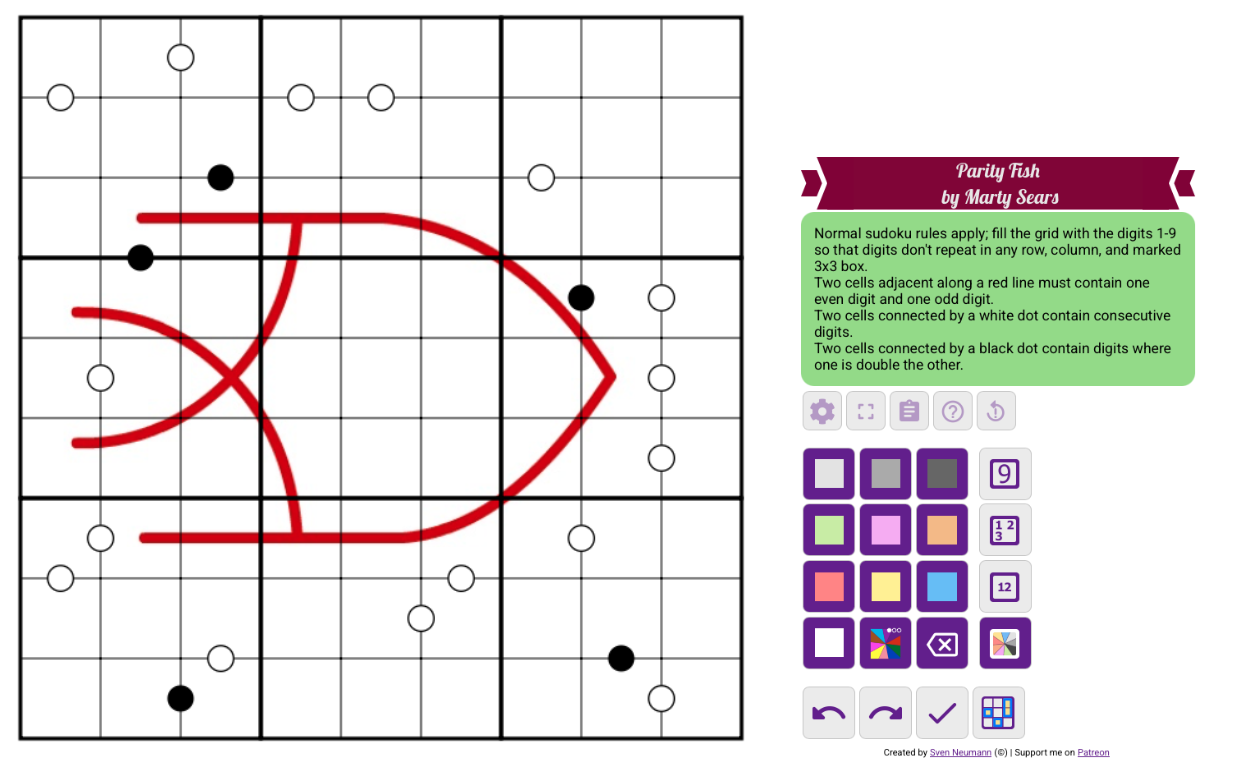
\includegraphics[width=8cm]{sakana_fish}
        \caption{Sakana Fish Puzzle}\label{fig:sakanaFish}
    \end{figure}

    In addition to the standard Sudoku rules,let us consider the constraints depicted in \figref{fig:sakanaFish}.

    \paragraph{Odd-even indicating hidden variables}
    The central hidden variable to be added is whether there is an even or odd digit at each position, denoted by $\headvariableof{r0,r1,c0,c1}$.
    We define the even checker as the function mapping even numbers to $1$ and odd to $0$, i.e.
    \begin{align*}
        E \defcols [\sudokunum^2] \rightarrow [2] \, .
    \end{align*}
    Now the even constraint is implemented
    \begin{align*}
        \bencodingofat{E}{\headvariableof{r0,r1,c0,c1},\decvariableof{r0,r1,c0,c1,:}}
        =& \tbasisat{\headvariableof{r0,r1,c0,c1}} \otimes \left(\sum_{i\in[\sudokunum^2] \wcols i \text{ is even}} \onehotmapofat{i}{\decvariableof{r0,r1,c0,c1,:}}\right) \\
        &+ \fbasisat{\headvariableof{r0,r1,c0,c1}} \otimes \left(\sum_{i\in[\sudokunum^2] \wcols i \text{ is odd}} \onehotmapofat{i}{\decvariableof{r0,r1,c0,c1,:}}\right) \, .
    \end{align*}

    \paragraph{Implementing red line constraints}
    Now along all pairs $(r0,r1,c0,c1),(\tilde{r0},\tilde{r1},\tilde{c0},\tilde{c1})$ the red lines we add constraint cores
    \begin{align*}
        \oplus\left[\headvariableof{r0,r1,c0,c1},\headvariableof{\tilde{r0},\tilde{r1},\tilde{c0},\tilde{c1}}\right]
    \end{align*}
    implementing the constraint, that odd-even digits are alternating.

    \paragraph{Implementing white dot constraints}
    These constraints can be implemented by cores to positions $(r0,r1,c0,c1),(\tilde{r0},\tilde{r1},\tilde{c0},\tilde{c1})$ connected via a white dot.
    The cores have coordinates
    \begin{align*}
        C^{\mathrm{white}}_{(r0,r1,c0,c1),(\tilde{r0},\tilde{r1},\tilde{c0},\tilde{c1})}\left[\indexeddecvariableof{r0,r1,c0,c1},\indexeddecvariableof{\tilde{r0},\tilde{r1},\tilde{c0},\tilde{c1}}\right]
        =\begin{cases}
             1 & \ifspace \absof{\decindexof{r0,r1,c0,c1}-\decindexof{\tilde{r0},\tilde{r1},\tilde{c0},\tilde{c1}}} = 1 \\
             0 & \text{else}
        \end{cases} \, .
    \end{align*}
    Note that they entail the constraints of red lines:
    \begin{align*}
        \oplus\left[\headvariableof{r0,r1,c0,c1},\headvariableof{\tilde{r0},\tilde{r1},\tilde{c0},\tilde{c1}}\right]
    \end{align*}

    \paragraph{Implementing black dot constraints}
    Analogously, the black dots can be implemented by
    \begin{align*}
        C^{\mathrm{black}}_{(r0,r1,c0,c1),(\tilde{r0},\tilde{r1},\tilde{c0},\tilde{c1})}\left[\indexeddecvariableof{r0,r1,c0,c1},\indexeddecvariableof{\tilde{r0},\tilde{r1},\tilde{c0},\tilde{c1}}\right]
        =\begin{cases}
             1 & \ifspace \decindexof{r0,r1,c0,c1}=2*\decindexof{\tilde{r0},\tilde{r1},\tilde{c0},\tilde{c1}} \\
             1 & \ifspace \decindexof{r0,r1,c0,c1}=0.5*\decindexof{\tilde{r0},\tilde{r1},\tilde{c0},\tilde{c1}} \\
             0 & \text{else}
        \end{cases} \, .
    \end{align*}
    Note that they entail the constraints (since at least one of the neighbors needs is even)
    \begin{align*}
        \lor\left[\headvariableof{r0,r1,c0,c1},\headvariableof{\tilde{r0},\tilde{r1},\tilde{c0},\tilde{c1}}\right] \, .
    \end{align*}
%

    \paragraph{Solution approach}
    Can we start the reasoning process by focusing only on the $\headvariableof{\cdot}$ variables?
    E.g. guess one, propagate on the rest and see if there is a contradiction.
%    \begin{align*}
%        \left(\headvariableof{r0,r1,c0,c1} \impbincon \headvariableof{\tilde{r0},\tilde{r1},\tilde{c0},\tilde{c1}}\right)
%        \lor
%        \left(\headvariableof{\tilde{r0},\tilde{r1},\tilde{c0},\tilde{c1}} \impbincon \headvariableof{r0,r1,c0,c1} \right)
%    \end{align*}


    \section{Toy Example for MCTS}

    As a toy example, let there be a knowledge base of atoms $A1$ and $A2$ representing two accounts to be used in an accounting proposal, and $E$ represents incoming invoices.
    The constraints are that exactly one of $A1$ or $A2$ is booked, that is $X_{A1}\oplus X_{A2}$.


    \begin{figure}[t]
        \centering
        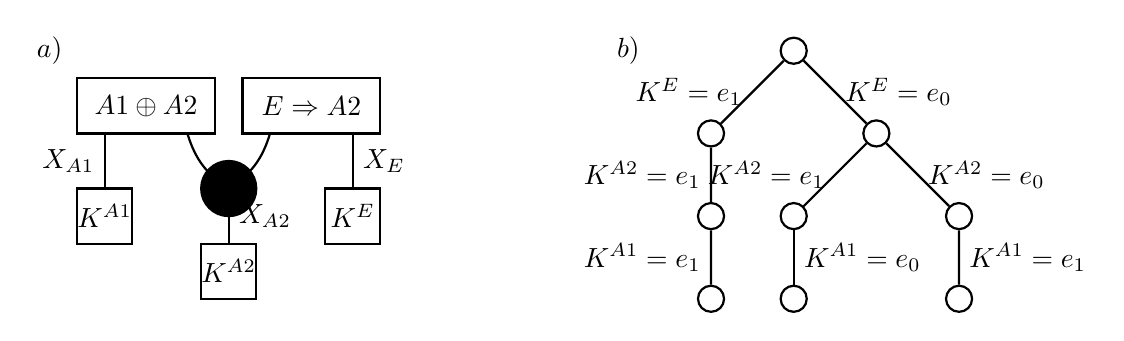
\begin{tikzpicture}[scale=0.35, thick]

            \node[anchor=center] (text) at (-2,0) {\corelabelsize $a)$};

            \draw (-1,-5) rectangle (1, -7);
            \node[anchor=center] (text) at (0,-6) {\corelabelsize $K^{A1}$};

            \draw[] (0,-3)--(0,-5)  node[midway,left] {\colorlabelsize $X_{A1}$};
            \draw[]  (3,-3) to[bend left = -20] (4.5,-5);
            \draw (-1,-1) rectangle (4, -3);
            \node[anchor=center] (text) at (1.5,-2) {\corelabelsize ${A1} \oplus {A2}$};

            \draw (5,-1) rectangle (10, -3);
            \node[anchor=center] (text) at (7.5,-2) {\corelabelsize $E \Rightarrow A2$};
            \draw (6,-3) to[bend left = 20] (4.5,-5);
            \draw[] (4.5,-5)--(4.5,-7) node[midway,right] {\colorlabelsize $X_{A2}$};
            \draw (3.5,-9) rectangle (5.5, -7);
            \node[anchor=center] (text) at (4.5,-8) {\corelabelsize $K^{A2}$};

            \draw[] (9,-3)--(9,-5) node[midway,right] {\colorlabelsize $X_E$};

            \draw (8,-5) rectangle (10, -7);
            \node[anchor=center] (text) at (9,-6) {\corelabelsize $K^{E}$};

            \draw[fill] (4.5,-5) circle (\dotsize);

            \begin{scope}
            [shift={(25,0)}]

                \node[anchor=center] (text) at (-6,0) {\corelabelsize $b)$};

                \node[draw, circle] (A) at (0,0) {};
                \node[draw, circle] (B) at (-3,-3) {};
                \node[draw, circle] (C) at (-3,-6) {};
                \node[draw, circle] (D) at (-3,-9) {};

                \node[draw, circle] (B1) at (3,-3) {};
                \node[draw, circle] (C1) at (0,-6) {};
                \node[draw, circle] (C2) at (6,-6) {};

                \node[draw, circle] (D1) at (0,-9) {};
                \node[draw, circle] (D2) at (6,-9) {};

                % Edges
                \draw (A) -- (B) node [midway, left] {\colorlabelsize $K^{E}=e_1$};
                \draw (A) -- (B1) node [midway, right] {\colorlabelsize $K^{E}=e_0$};
                \draw (B) -- (C) node [midway, left] {\colorlabelsize $K^{A2}=e_1$};
                \draw (C) -- (D) node [midway, left] {\colorlabelsize $K^{A1}=e_1$};

                \draw (B1) -- (C1) node [midway, left] {\colorlabelsize $K^{A2}=e_1$};
                \draw (B1) -- (C2) node [midway, right] {\colorlabelsize $K^{A2}=e_0$};

                \draw (C1) -- (D1) node [midway, right] {\colorlabelsize $K^{A1}=e_0$};
                \draw (C2) -- (D2) node [midway, right] {\colorlabelsize $K^{A1}=e_1$};

            \end{scope}

        \end{tikzpicture}
        \caption{a) Tensor Network Representation of a toy CSP, in which two formulas ${A1} \oplus {A2}$ and $E\Rightarrow {A2}$ have to be satisfied.
        The Knowledge Cores $K$ contain the possible choices after a constraint propagation and are taken from $e_0,e_1,\underline{1},\underline{0}$.
        b) The corresponding search tree, where the assignments to variables are guessed in the order $E,{A2},{A1}$.
        At each parent with a single child, the other choice has been ruled out by constraint propagation.
        In our toy example with minimally connected constraints, single-core constraint propagation ensures that the guessed reasoning path remains consistent.}
    \end{figure}

    \bibliographystyle{plainnat}
    \bibliography{../../references.bib}

\end{document}